\documentclass[border=6pt]{standalone}
\usepackage{tikz}
\usepackage{amsmath,amssymb}
\usepackage{xcolor}
\usetikzlibrary{arrows.meta,positioning,fit,backgrounds,calc,decorations.pathreplacing}
\definecolor{cBlue}{HTML}{CBDCF3}
\definecolor{cBlueL}{HTML}{5B86C9}
\definecolor{cGreen}{HTML}{CBE8D3}
\definecolor{cGreenL}{HTML}{5BA772}
\definecolor{cGray}{HTML}{ECEEF1}
\definecolor{cGrayL}{HTML}{9AA2AC}
\definecolor{cStage}{HTML}{D4ECF0}
\definecolor{cStageL}{HTML}{4FA3B3}
\definecolor{cState}{HTML}{FBE7C4}
\definecolor{cStateL}{HTML}{E0A647}
\definecolor{cAgent}{HTML}{E3D4F3}
\definecolor{cAgentL}{HTML}{8A5CC2}
\definecolor{cFin}{HTML}{E3E7EC}
\definecolor{cAccent}{HTML}{D1495B}

\begin{document}
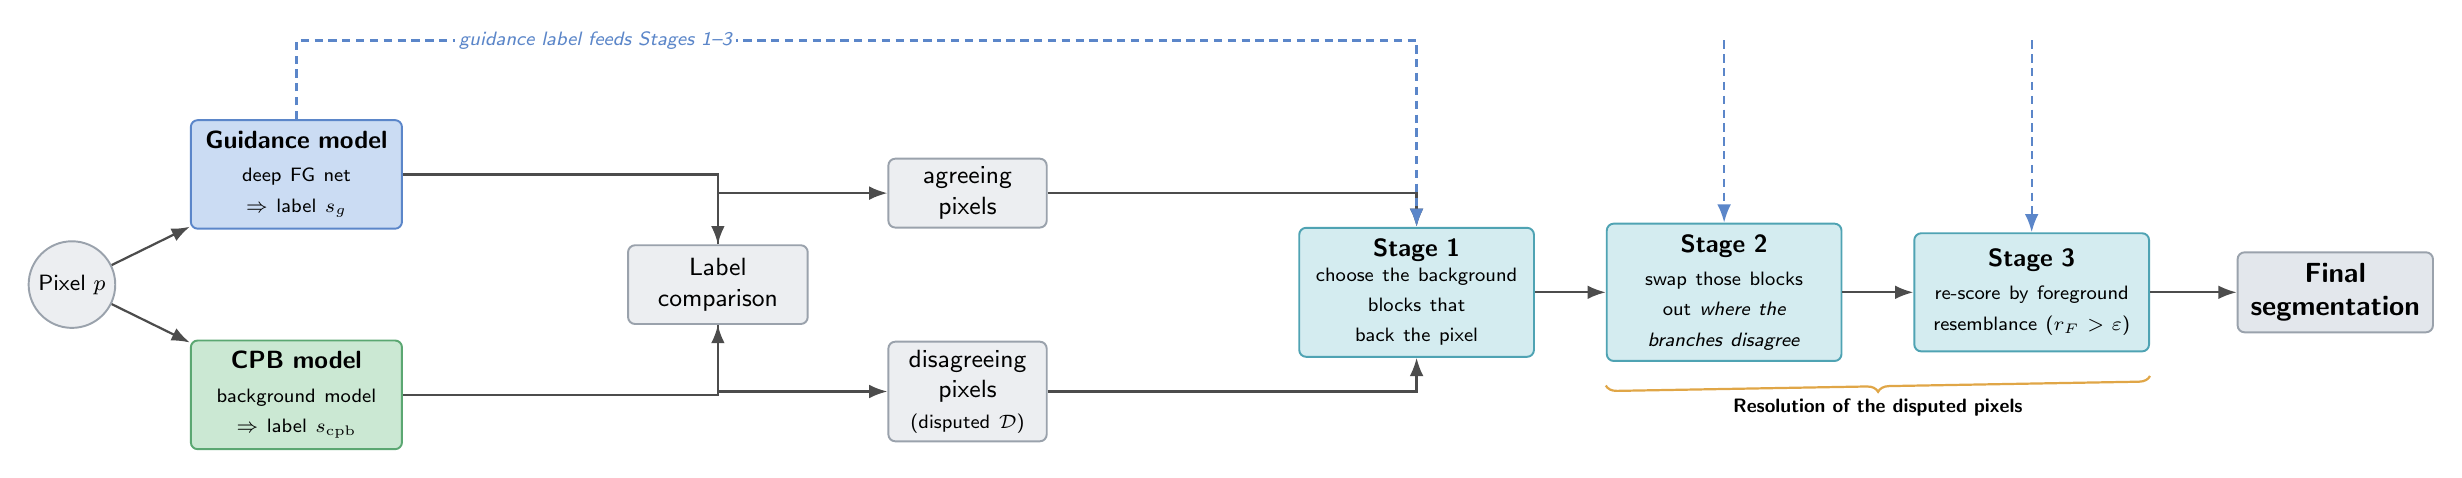
\begin{tikzpicture}[
  >=Latex, font=\sffamily\small, node distance=7mm, line width=0.7pt,
  box/.style   ={draw=cGrayL, rounded corners=2.5pt, align=center, minimum height=10mm,
                 inner sep=4pt, fill=cGray},
  guid/.style  ={box, fill=cBlue,  draw=cBlueL,  text width=24mm},
  cpb/.style   ={box, fill=cGreen, draw=cGreenL, text width=24mm},
  small/.style ={draw=cGrayL, rounded corners=2.5pt, align=center, fill=cGray,
                 inner sep=3pt, minimum height=8mm, text width=18mm},
  stage/.style ={draw=cStageL, rounded corners=2.5pt, align=center, fill=cStage,
                 inner sep=4pt, minimum height=15mm, text width=27mm},
  pix/.style   ={draw=cGrayL, circle, align=center, fill=cGray, inner sep=1pt,
                 minimum size=11mm, font=\sffamily\footnotesize},
  fin/.style   ={box, fill=cFin, draw=cGrayL, font=\sffamily\bfseries, text width=22mm},
  e/.style     ={->, thick, draw=black!70},
  g/.style     ={->, thick, cBlueL, densely dashed},
  lbl/.style   ={font=\sffamily\scriptsize\itshape, inner sep=1.5pt}]

  \node[pix] (pix) {Pixel $p$};
  \node[guid, above right=3mm and 11mm of pix] (guid) {\textbf{Guidance model}\\[1pt]\scriptsize deep FG net $\Rightarrow$ label $s_g$};
  \node[cpb, below right=3mm and 11mm of pix]  (cpb)  {\textbf{CPB model}\\[1pt]\scriptsize background model $\Rightarrow$ label $s_{\mathrm{cpb}}$};
  \node[box, right=12mm of pix, text width=20mm] (cmp) at ($(guid)!0.5!(cpb)+(30mm,0)$) {Label\\comparison};

  \node[small, above right=2mm and 10mm of cmp] (agr) {agreeing\\pixels};
  \node[small, below right=2mm and 10mm of cmp] (dis) {disagreeing\\pixels\\{\scriptsize(disputed $\mathcal{D}$)}};

  \node[stage, right=12mm of cmp] (s1) at ($(agr)!0.5!(dis)+(30mm,0)$)
       {\textbf{Stage 1}\\[1pt]\scriptsize choose the background\\blocks that back the pixel};
  \node[stage, right=9mm of s1] (s2)
       {\textbf{Stage 2}\\[1pt]\scriptsize swap those blocks out \emph{where the branches disagree}};
  \node[stage, right=9mm of s2] (s3)
       {\textbf{Stage 3}\\[1pt]\scriptsize re-score by foreground resemblance ($r_F>\varepsilon$)};
  \node[fin, right=11mm of s3] (out) {Final\\segmentation};

  % main edges
  \draw[e] (pix) -- (guid);
  \draw[e] (pix) -- (cpb);
  \draw[e] (guid) -| (cmp);
  \draw[e] (cpb)  -| (cmp);
  \draw[e] (cmp) |- (agr);
  \draw[e] (cmp) |- (dis);
  \draw[e] (agr) -| (s1);
  \draw[e] (dis) -| (s1);
  \draw[e] (s1) -- (s2);
  \draw[e] (s2) -- (s3);
  \draw[e] (s3) -- (out);

  % guidance label feeds every stage (top rail)
  \coordinate (top) at ($(guid.north)+(0,10mm)$);
  \draw[g] (guid.north) |- (top) -| (s1.north);
  \draw[g] (top -| s2.north) -- (s2.north);
  \draw[g] (top -| s3.north) -- (s3.north);
  \node[lbl, cBlueL, fill=white] at ($(top)+(38mm,0)$) {guidance label feeds Stages 1--3};

  % bracket over stage 2--3
  \draw[thick, cStateL, decorate, decoration={brace, amplitude=4pt, mirror}]
       ($(s2.south west)+(0,-3mm)$) -- ($(s3.south east)+(0,-3mm)$)
       node[midway, below=3pt, font=\sffamily\scriptsize\bfseries, text=black]{Resolution of the disputed pixels};
\end{tikzpicture}
\end{document}
